\documentclass[12pt]{article}
\usepackage{graphicx,graphics}
\usepackage{amsmath}
\usepackage{amssymb}
\usepackage{epstopdf}
\usepackage{amstext}
\usepackage{amsthm}
\usepackage{amsfonts}
\usepackage{latexsym}
\usepackage{array}
\usepackage{xfrac}
\usepackage{color}
\usepackage[spanish]{babel}
\usepackage{amsmath}
\title{\ De la ecuaci\'on de Schrodinger a Gross-Pitaevskii}
\date{}
% Este es un comentario, no será mostrado en el documento final.
\begin{document}
\maketitle 
\section{Introducci\'on a la Mec\'anica Cu\'antica}
\section{Soluciones a la ecuaci\'on de Schrodinger}
En esta secci\'on estudiaremos soluciones a la ecuación de Schrodinger.
\begin{align}
i\hbar\frac{\partial}{\partial t}
\Psi =\left(-\hbar^2/2m \,\vec{\nabla}^2+V_{\rm trap}(r) 
\right)\Psi
\label{eq:schr}
\end{align}
\subsection{Movimiento libre}
Primero analizaremos la ec. ~\eqref{eq:schr} imponiendo que $V_{trap}=0$, por tanto nos queda una ecuaci\'on:
\begin{align}
i\hbar\frac{\partial}{\partial t}
\Psi =\left(-\hbar^2/2m \,\vec{\nabla}^2 
\right)\Psi
\label{eq:schr_free}
\end{align}
 en este caso podemos hacer una analog\'ia al movimiento libre de una part\'cula. Podemos comprobar que dado este sistema el Hamiltoniano conmuta con el operador momento $p=-i\hbar\vec{\nabla}$, por lo tanto si hacemos la transformada de Fourier de nuestro paquetes de ondas debe ser un estado propio de nuestro sistema, por el cual no observaremos dispersi\'on.
 \begin{align}
 \Psi(k) =\sqrt{\frac{1}{2\pi}} \,\int_{-\infty}^{\infty}\Psi(x)e^{-ikx}dx
 \label{eq:four}
 \end{align}
 
 En mec\'anica cu\'antica el valor medio de un operador $A$ se define como:
 \begin{align}
 \ <A>=\int_{-\infty}^{\infty}\Psi^{*}(x)A\Psi(x) dx
 \label{eq:mean}
 \end{align}
 As\'i la dispersi\'on del operador $A$ la definimos como: $ \sigma=\sqrt{<A^2>-<A>^2}  $
 \\
 
\subsection{Oscilador arm\'onico}
En este punto introduciremos un potencial externo a la ecuaci\'on de Schrodinger, que ser\'a el famoso potencial arm\'onico:  $V_{trap}=\dfrac{1}{2}mw^2x^2$.

Nuestro objetivo ser\'a obtener las autofunciones y autovalores del Hamiltoniano, para ello resolvemos la ecuaci\'on ~\eqref{eq:schr}. No nos centraremos en el m\'etodo a seguir para encontrar esta soluciones, simplemente mencionamos que se pueden obtener llevando un desarrollo en serie de potencias. As\'i obtenemos la fam\'ilia de soluciones:

 \begin{align}
\psi_n(x)=\sqrt{\frac{1}{2^n n!}} (\dfrac{mw}{\pi\hbar})^{1/4}\exp(\dfrac{mwx^2}{2\hbar})H_n(\sqrt{\frac{mw}{\hbar}}x) \,\,\,\,\,\,\,\ n=0,1,2,...
\label{eq:sol_schr}
\end{align}

donde $H_n$ son los polinomios de Hermite:

\begin{align}
H_n(x)=(-1)^n e^{x^2} \dfrac{d^n}{dx^n}e^{-x^2}
\label{eq:herm}
\end{align}

Y obtenemos unos niveles de energ\'ia:

\begin{align}
E_n=\hbar w(n+\dfrac{1}{2})
\label{eq:energ}
\end{align}

Este resultado es muy importante en la mec\'anica cu\'antica. Ya que nos muestra una cuantizaci\'on en la energ\'ia, as\' que tendremos distintos niveles de energ\'ia posibles en nuestro estado.
\pagebreak

\section{Simulaci\'on: ecuaci\'on de Schrodinger}
\subsection{Movimiento libre}
Para inicializar la simulaci\'on donde veremos soluciones a la ec. \eqref{eq:schr} entramos en la secci\'on \textit{WavePack Dispersion}.

Para observar un movimiento libre seleccionamos el bot\'on \textit{No} en \textit{Harmonic}, con el slider \textit{Initial position Wavepack} podemos seleccionar la posici\'on inicial de nuestro paquete de ondas. En \textit{excitation of the state} seleccionamos uno de los autoestados dados por la ec. \eqref{eq:sol_schr} y \textit{Number of oscilations} nos permite controlar el tiempo de la simulaci\'on, este tiempo est\'a escalado con el periodo del paquete de ondas bajo un potencial de $w=1$, ahora seleccionamos el bot\'on \textit{START}. Una vez terminada la computaci\'on, principalmente nos interesar\'a la ventana \textit{DISPERSION}. En ella se muestra el c\'alculo de la dispersi\'on para la funci\'on de onda en el espacio R y K, vemos como incrementa con el tiempo para R y constante para K. Seguidamente podemos ver la evoluci\'on de nuestro estado. Utilizando el slider debajo de la gr\'afica o los botones \textit{GO ON, GO BACK, PAUSE} podemos controlar la evoluci\'on del estado. Vemos como ciertamente nuestra funci\'on de onda en el espacio K no sufre ning\'un tipo de dispersi\'on pero en el espacio R s\'i.

\subsection{Oscilador arm\'onico}

Para activar el movimiento oscilatorio arm\'onico solamente debemos presionar el bot\'on \textit{YES} en \textit{HARMONIC}. En esta secci\'on nos centraremos en dos puntos:
\\

(I) Comprobar que el paquete de ondas sigue un movimiento oscilatorio arm\'onico.

(II) Comprobar la cuantizaci\'on de la energ\'ia dada por la ec.  ~\eqref{eq:energ}.
\\

Para obtener los resultados del apartado (I) posicionaremos el paquete de ondas en una posici\'on diferente de 0, se puede elegir el nivel de excitaci\'on que uno desee y ejecutaremos el programa para un tiempo dado. Una vez haya terminado la computaci\'on podemos seleccionar la gr\'afica\textit{ ENERGY}. En ella podemos ver tres valor de la energ\'ia: cin\'etica, potencial y total. Podemos observar una oscilaci\'on como la que cumplir\'ia una part\'icula bajo un potencial arm\'onico, como la de la Fig.~\ref{Fig:harm} . Ahora entramos en la evoluci\'on del estado, ya se ha comentado anteriormente como entrar. En \'el, podemos ver completamente un movimiento oscilatorio. Vemos que, cuando la funci\'on de onda en el espacio R est\'a en un extremo, en el espacio K est\'a en 0 y a la inversa, muestra de un movimiento oscilatorio. En este punto uno ser\'ia capaz de extraer el per\'iodo del movimiento entrando en \textit{MEAN VALUE} donde est\'a calculado el valor medio de la posici\'on del paquete siguiendo la ec ~\eqref{eq:mean} y as\'i compararlo con el resultado te\'orico.
\linebreak

\begin{figure}[tb]
	\centering
	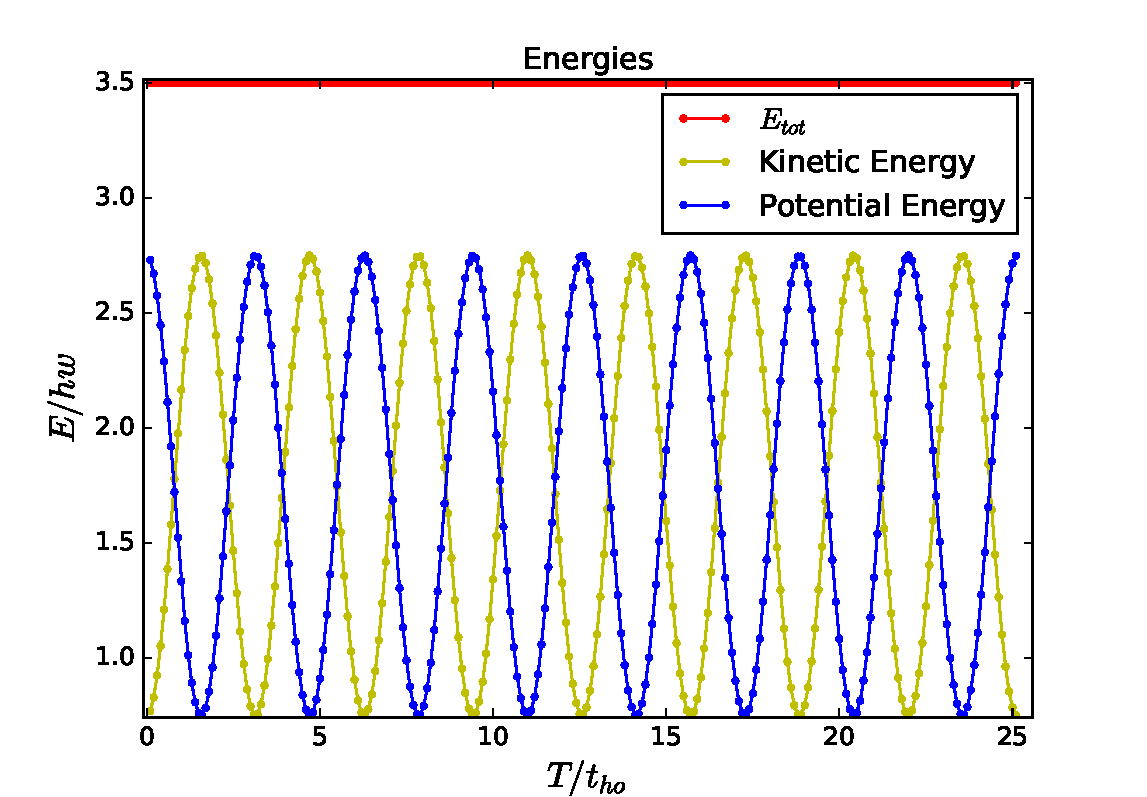
\includegraphics[width=0.9\linewidth]{harm.pdf}
	\caption{Energ\'ias para una funci\'on de onda sometida a un potencial arm\'onico}
	\label{Fig:harm}
\end{figure}
Ahora analicemos el punto (II). La configuraci\'on inicial adecuada ser\'ia: poner el paquete de ondas en la posici\'on 0, introducir un tiempo que queramos y, lo m\'as importante seleccionar el nivel de excitaci\'on, empezaremos con el nivel 0. Una vez finalizados los c\'alculos entramos en \textit{ENERGY}, esta vez, nos interesa la energ\'ia total. Ahora podemos comparar este valor con el dado por la ec. ~\eqref{eq:energ} para $n=0$, ahora reiteramos para $n=1,2$. Tambi\'en podemos comprobar viendo la evoluci\'on del estado que es un propio y por lo tanto, estacionario.

\section{Gross-Pitaevskii (r\'egimen No-lineal)}

\subsection{Condensados de Bose-Einstein y ecuaci\'on de Gross-Pitaevskii}
Los bosones est\'an caracterizados por no cumplir el principio de exclusi\'on de Pauli, es decir, distintos bosones pueden ocupar el mismo estado cu\'antico, totalmente opuesto a los fermiones. Cuando se tiene un sistema bos\'onico, y a \'este se le disminuye la temperatura hasta llegar cerca del 0 absoluto (-273.15 ºC) forman un nuevo estado de la materia llamado la condensaci\'on de Bose-Einstein. Se caracteriza por la ocupaci\'on ,de una gran parte de la fracci\'on de bosones, del estado cu\'antico fundamental. Este fen\'omeno nos lleva a tener un estado cu\'antico macr\'oscopico, donde podemos caracterizar nuestro sistema por una \'unica funci\'on de onda.
\\

Dado este sistema de $N$ bosones. Si ahora consideramos que la interacci\'on entre los bosones es de contacto entre dos cuerpos, y que la separaci\'on entre dos bosones es mayor que la \textit{scattering lenght}, podemos efectuar la siguiente aproximaci\'on:
 
\begin{align}
\psi(\mathbf{r_1,r_2,...,r_N})=\psi(\mathbf{r_1})\psi(\mathbf{r_2})...\psi(\mathbf{r_N})
\label{eq:aprox}
\end{align}

Con esto podemos escribir nuestro Hamiltoniano de la forma siguiente:

\begin{align}
H=\sum_{i=1}^{N}(-\frac{\hbar}{2m}\frac{\partial^2}{\partial\mathbf{r_i^2}}+V_{trap}(\mathbf{r_i}))+\sum_{i<j}\frac{4\pi \hbar^2 a_s}{m}
\delta(\mathbf{r_i-r_j})
\label{eq:hamGP}
\end{align}

Donde $m$ es la masa de de un bos\'on, $a_s$ es la \textit{boson-boson scattering lenght} y $delta(\mathbf{r})$ es la delta de Dirac.

En este punto podemos escribir la ecuaci\'on de Gross-Pitaevskii (independiente del tiempo):

\begin{align}
 \mu
\Psi(\mathbf{r}) =\left(-\frac{\hbar^2}{2m} \,\vec{\nabla}^2+V_{\rm trap}(\mathbf{r})+g|\Psi(\mathbf{r})|^2 
\right)\Psi(\mathbf{r})
\label{eq:GP}
\end{align}

Donde $g=\frac{4\pi \hbar^2 a_s}{m}$ que es proporcional al \textit{scattering lenght} y  $\mu$ es el potencial qu\'imico. El cual se puede encontrar con la condici\'on de normalizaci\'on de la funci\'on de onda:

\begin{align}
N=\int |\Psi(\mathbf{r})|^2 d^3r
\label{eq:norma}
\end{align}

Vemos como la ecuaci\'on de Gross-Pitaevskii es una ecuaci\'on diferencial no-lineal. Vemos que la no-linealidad la introduce el t\'ermino que va con $g$. Por tanto, vemos que para el caso $g=0$ recuperamos la ec. ~\eqref{eq:schr}, lo que nos lleva a que las soluciones de la ecuaci\'on de Gross-Pitaevskii son la continuaci\'on no-lineal de las de Schrodinger.

\subsection{Aproximaci\'on Thomas-Fermi y solitones oscuros}
Apartir de ahora supondremos un r\'egimen 1D. La primera soluci\'on que podemos hallar en la ec.~\eqref{eq:GP}  es haciendo la aproximaci\'on siguiente:
Suponemos tener un gran n\'umero de part\'iculas, lo que lleva a que el t\'ermino interat\'omico se haga muy grande, as\'i podemos despreciar el t\'ermino cin\'etico. Una vez hecho esto, la ecuaci\'on a resolver es trivial, con soluci\'on:
 
 \begin{align}
 \psi(x)=\sqrt{\frac{\mu-V_{trap}(x)}{gN}}
 \label{eq:TF}
 \end{align}
 
Otro tipo de soluci\'on a la ec.~\eqref{eq:GP}  son los solitones. Depende del tipo de interaci\'on, si es atractiva o repulsiva podemos tener solitones brillantes o oscuros, respectivamente. Para una interacci\'on repulsiva tenemos:

 \begin{align}
\psi(x)=\psi_0 \tanh{\frac{x}{\sqrt{2}\xi}}
\label{eq:soliton}
\end{align}

Donde $\psi_0$ es la soluc\'on a la ec.~\eqref{eq:GP} sin solit\'on y $\xi=\frac{\hbar}{\sqrt{2mgN}}$ es la llamada \textit{healing length}
\\

Esta \'ultima soluci\'on tiene un especial inter\'es. Vemos que los solitones oscuros producen un punto de cero densidad. Estos objetos son un defecto topol\'ogico del sistema, se puede observar que producen un cambio en la funci\'on de onda. En concreto, producen un salto de fase $\pi$ en el punto donde se hallan.
\\

\subsection{Solitones Oscuros bajo un potencial arm\'onico}
\subsection{P\'endulo de Newton cu\'antico}

\section{Simulaci\'on: GP-ecuaci\'on}
\subsection{Continuaci\'on no-lineal}
En esta secci\'on se comprobaremos que las soluciones a la ec.~\eqref{eq:GP} simplemente son una continuaci\'on no-lineal de las soluciones a la ec.~\eqref{eq:schr}. Es decir, que haciendo tender $g\rightarrow0$ recuperamos las soluciones lineales. Para ello entramos en la simulaci\'on \textit{DarkSolitons}. Nada m\'as entrar podemos observar un condensado de Bose-Einstein para $\mu=42$ y su aproximaci\'on Thomas-Fermi. Apretamos el bot\'on \textit{Lineal continuation} y veremos que se desplega una caja donde seleccionar el n\'umero de excitaci\'on. Es decir, recordando la cuantizaci\'on de la energ\'ia ~\eqref{eq:energ}, podemos seleccionar el estado lineal con el cual queremos observar la evoluci\'on de la no-linealidad. una vez terminado el tiempo de computaci\'on, podemos presionar sobre \textit{CHEMICAL POTENTIAL}. En esta gr\'afica podemos observar el valor del potencial qu\'imico a medida que augmentamos el valor de $g_{int}$. Podemos comprobar que para valores nulos de la no-linealidad recuperamos el resultado predecido por la ec.  ~\eqref{eq:energ}. El m\'etodo para entrar en la evoluci\'on del estado es el mismo que en la simulaci\'on \textit{WavePackDispersion}. Aqu\'i veremos como nuestro estado evoluciona a medida que aumentamos el valor de $g_{int}$, es decir, tenemos una visi\'on directa de como afecta la no-linealidad de nuestro estado. Este proceso se puede iterar para las diferentes excitaciones posibles que da el programa. As\'i, recopilando los datos, podemos obtener una figura como la Fig.~\ref{Fig:cont_lin}


\begin{figure}[tb]
	\centering
	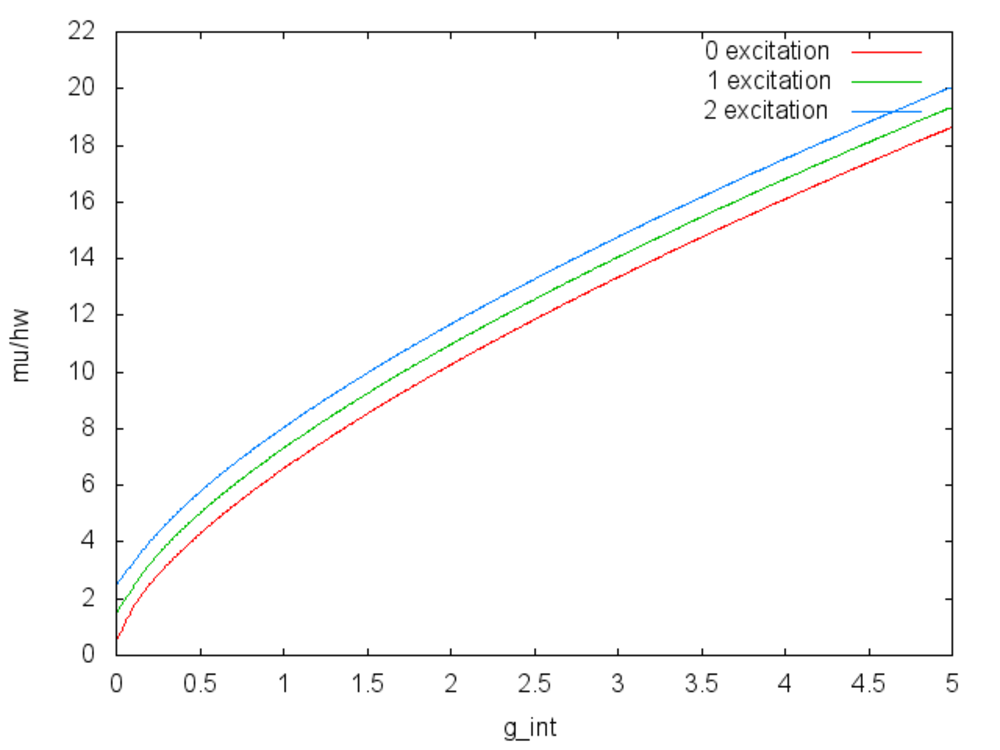
\includegraphics[width=0.9\linewidth]{cont_lin.pdf}
	\caption{Potencial qu\'imico para diferentes estados en su evoluci\'on en la no-linealidad}
	\label{Fig:cont_lin}
\end{figure}

\subsection{Solit\'on oscuro bajo un potencial arm\'onico}
Ahora veremos el comportamiento de estos defectos topol\'ogicos bajo un potencial arm\'onico. Como hemos visto estos objetos se comportan como una part\'icula con una masa asociada (negativa), aqu\'i comprobaremos este hecho. En primer lugar presionamos el bot\'on \textit{Dark solitons study}. Introducimos la posici\'on inicial del solit\'on, el n\'umero de oscilaciones que queremos que de e introduciremos en \textit{Number of symmetric solitons = 1}. Presionamos ahora el bot\'on \textit{START} y esperamos a que finalice el tiempo de computaci\'on. Ahora podemos entrar en el apartado \textit{MINUS}, en el vemos una gr\'afica donde se representa nuestro condensado para diferentes instantes de tiempo. En el podemos extraer el periodo de oscilaci\'on de nuestro solit\'on y con el podr\'iamos extraer su masa asociada. En el apartado \textit{PHASE} podemos comprobar que un solit\'on es un defecto topol\'ogico. En esta gr\'afica se representa la diferencia de fase entre la parte derecha del solit\'on y la parte izquierda, como se ha mencionado en teor\'ia, se introduce un cambio de fase $\pi$ pero como el solit\'on al oscilar adquiere velocidad este ya no introduce un 0 en la densidad, por lo tanto este cambio de fase es menor. Por \'ultimo podemos entrar en la evoluci\'on del estado y veremos como el solit\'on oscila con el tiempo.

\subsection{Interacci\'on entre dos solitones oscuros bajo un potencial arm\'onico}
 Como ya se ha mencionado, la interacci\'on entre dos solitones es repulsiva, ahora comprobaremos esta interacci\'on en presencia de un potencial arm\'onico. Para observar este fen\'omeno introducimos los mismos par\'ametros que en el apartado anterior pero ahora, seleccionaremos \textit{Number of symmetric solitons = 2}. Lo que calcularemos ahora es una soluci\'on con dos solitones impresos de forma sim\'etrica. Primero ejecutamos el programa con una posici\'on entre ellos mayor a 2. Podemos comprobar en el apartado \textit{MINUS} como el periodo es exactamente el mismo que con solo un solit\'on. Ha medida que hagamos los c\'alculos con una posici\'on mas pequeña entre ellos, veremos como el periodo se va reduciendo. A una poisici\'on muy pequeña veremos un r\'egimen totalmente repulsivo entre los solitones (recuperamos la interacci\'on para un background homogéneo). Podemos encontrar un estado ligado entre estos donde tendríamos una soluci\'on estacionaria con los solitones, como la que vemos en la Fig.~\ref{Fig:stati_3}. Es interesante recoger diversos valores del periodo para diferentes posiciones de los solitones, obtendr\'iamos una gr\'afica como la que se muestra en la Fig.~\ref{Fig:per}. No podemos recuperar con esta simulaci\'on un fuerte resultado (podr\'iamos pero el m\'etodo ser\'ia extensamente largo), que es que la energ\'ia de interacci\'on entre dos solitones es muy similar al potencial tipo part\'icula.
 
  \begin{figure}[tb]
 	\centering
 	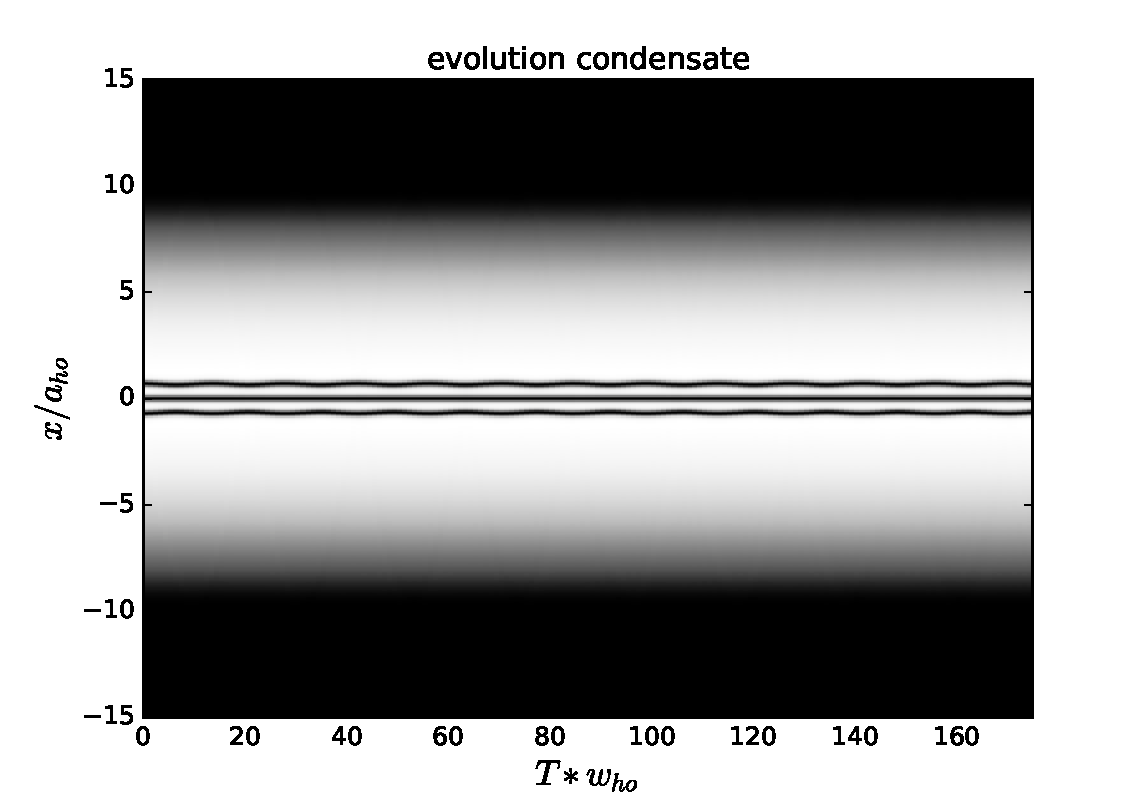
\includegraphics[width=0.9\linewidth]{stati_3.pdf}
 	\caption{Estado ligado para 3 solitones oscuros.}
 	\label{Fig:stati_3}
 \end{figure}
 
 \begin{figure}[tb]
 	\centering
 	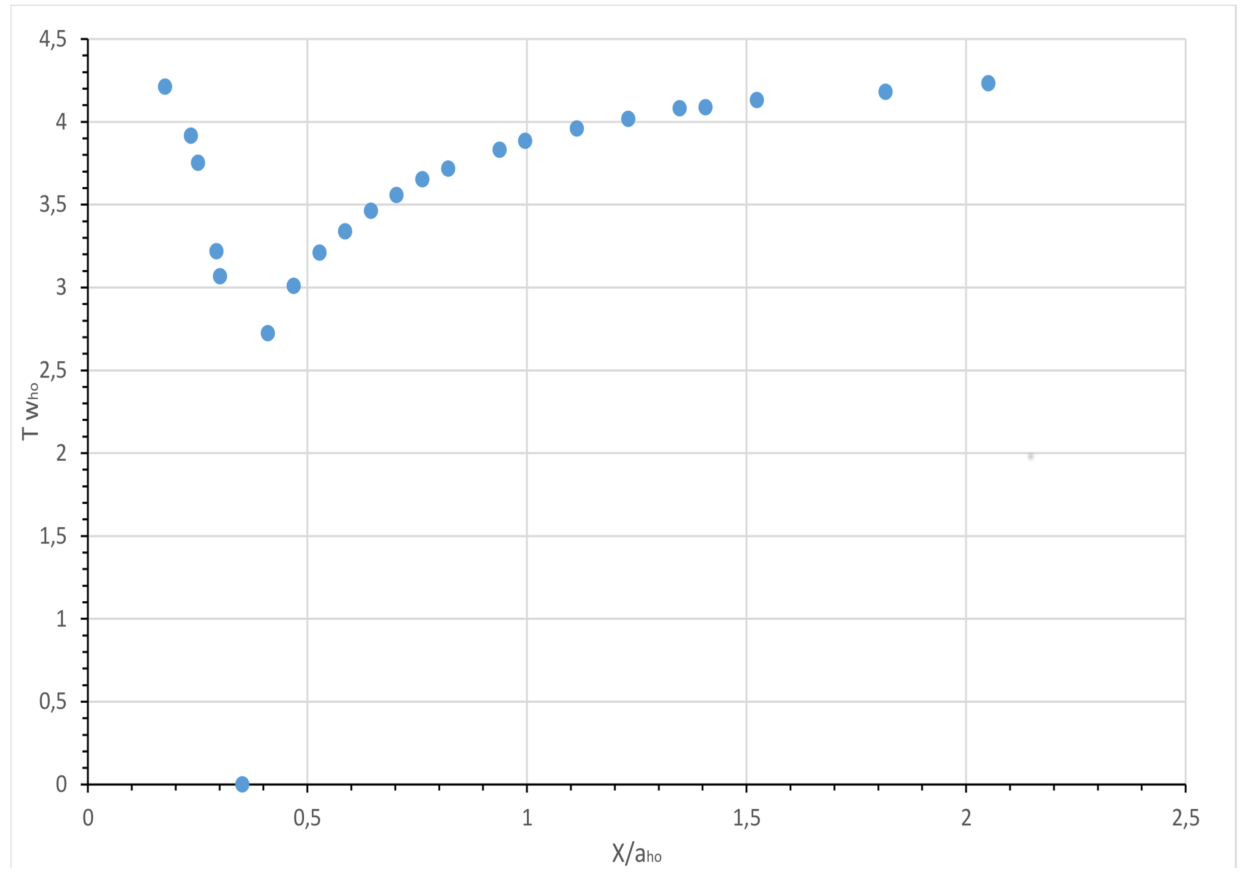
\includegraphics[width=0.9\linewidth]{periodo.pdf}
 	\caption{Evoluci\'on del periodo de dos solitones para diferentes posiciones sim\'etricas de estos}
 	\label{Fig:per}
 \end{figure}

\subsection{P\'endulo de Newton con solitones}
Ahora que hemos estudiado diferentes propiedades de los solitones oscuros y la condensaci\'on de Bose-Einstein, vamos a proceder con un ejemplo bastante interesante donde mezclaremos diversos conceptos utilizados.

Para inicializar este proceso debemos clicar en el m\'odulo \textit{Newton's cradle}, en \textit{Computation control} se nos abrir\'an diferentes comandos a controlar. B\'asicamente controlaremos dos estados, uno ser\'a el estado central sim\'etrico al que llamaremos la cadena de solitones; el otro ser\'a un estado que chocar\'a con el anterior, que ser\'a el estado inicialmente en movimiento. En \textit{number of solitons in motion} podemos controlar el n\'umero de solitones que queremos en el estado en movimiento (de 1 a 2). En \textit{initial position of solitons in motion} controlamos la posici\'on inicial de este mismo estado. Con \textit{number of oscilations} controlamos el tiempo total que durar\'a la simulaci\'on, b\'asicamente est\'a escalado con el periodo que tiene un \'unico solit\'on. Finalmente con \textit{number of solitons in chair} controlamos el estado central sim\'etrico estacionario, podemos seleccionar de cu\'antos solitones est\'a formado (de 1 a 3). Una vez est\'en todas las configuraciones seleccionadas iniciamos la simulaci\'on. 

En este m\'odulo nos interesaremos en la evoluci\'on del estado y en la gr\'afica \textit{MINUS}, donde podemos obtener gr\'aficas como la mostrada en la Fig.~\ref{Fig:new_crand}. Podemos observar un claro s\'imil con un fen\'omeno del mundo cl\'asico, el p\'endulo de Newton. No olvidemos que lo que tenemos aqu\'i es un condensado de Bose-Einstein y solitones oscuros. Sin embargo podemos ver que el comportamiento de estos es muy parecido al que tendr\'ian unas bolas con un volumen y masa bajo un potencial. 

\begin{figure}[tb]
	\centering
	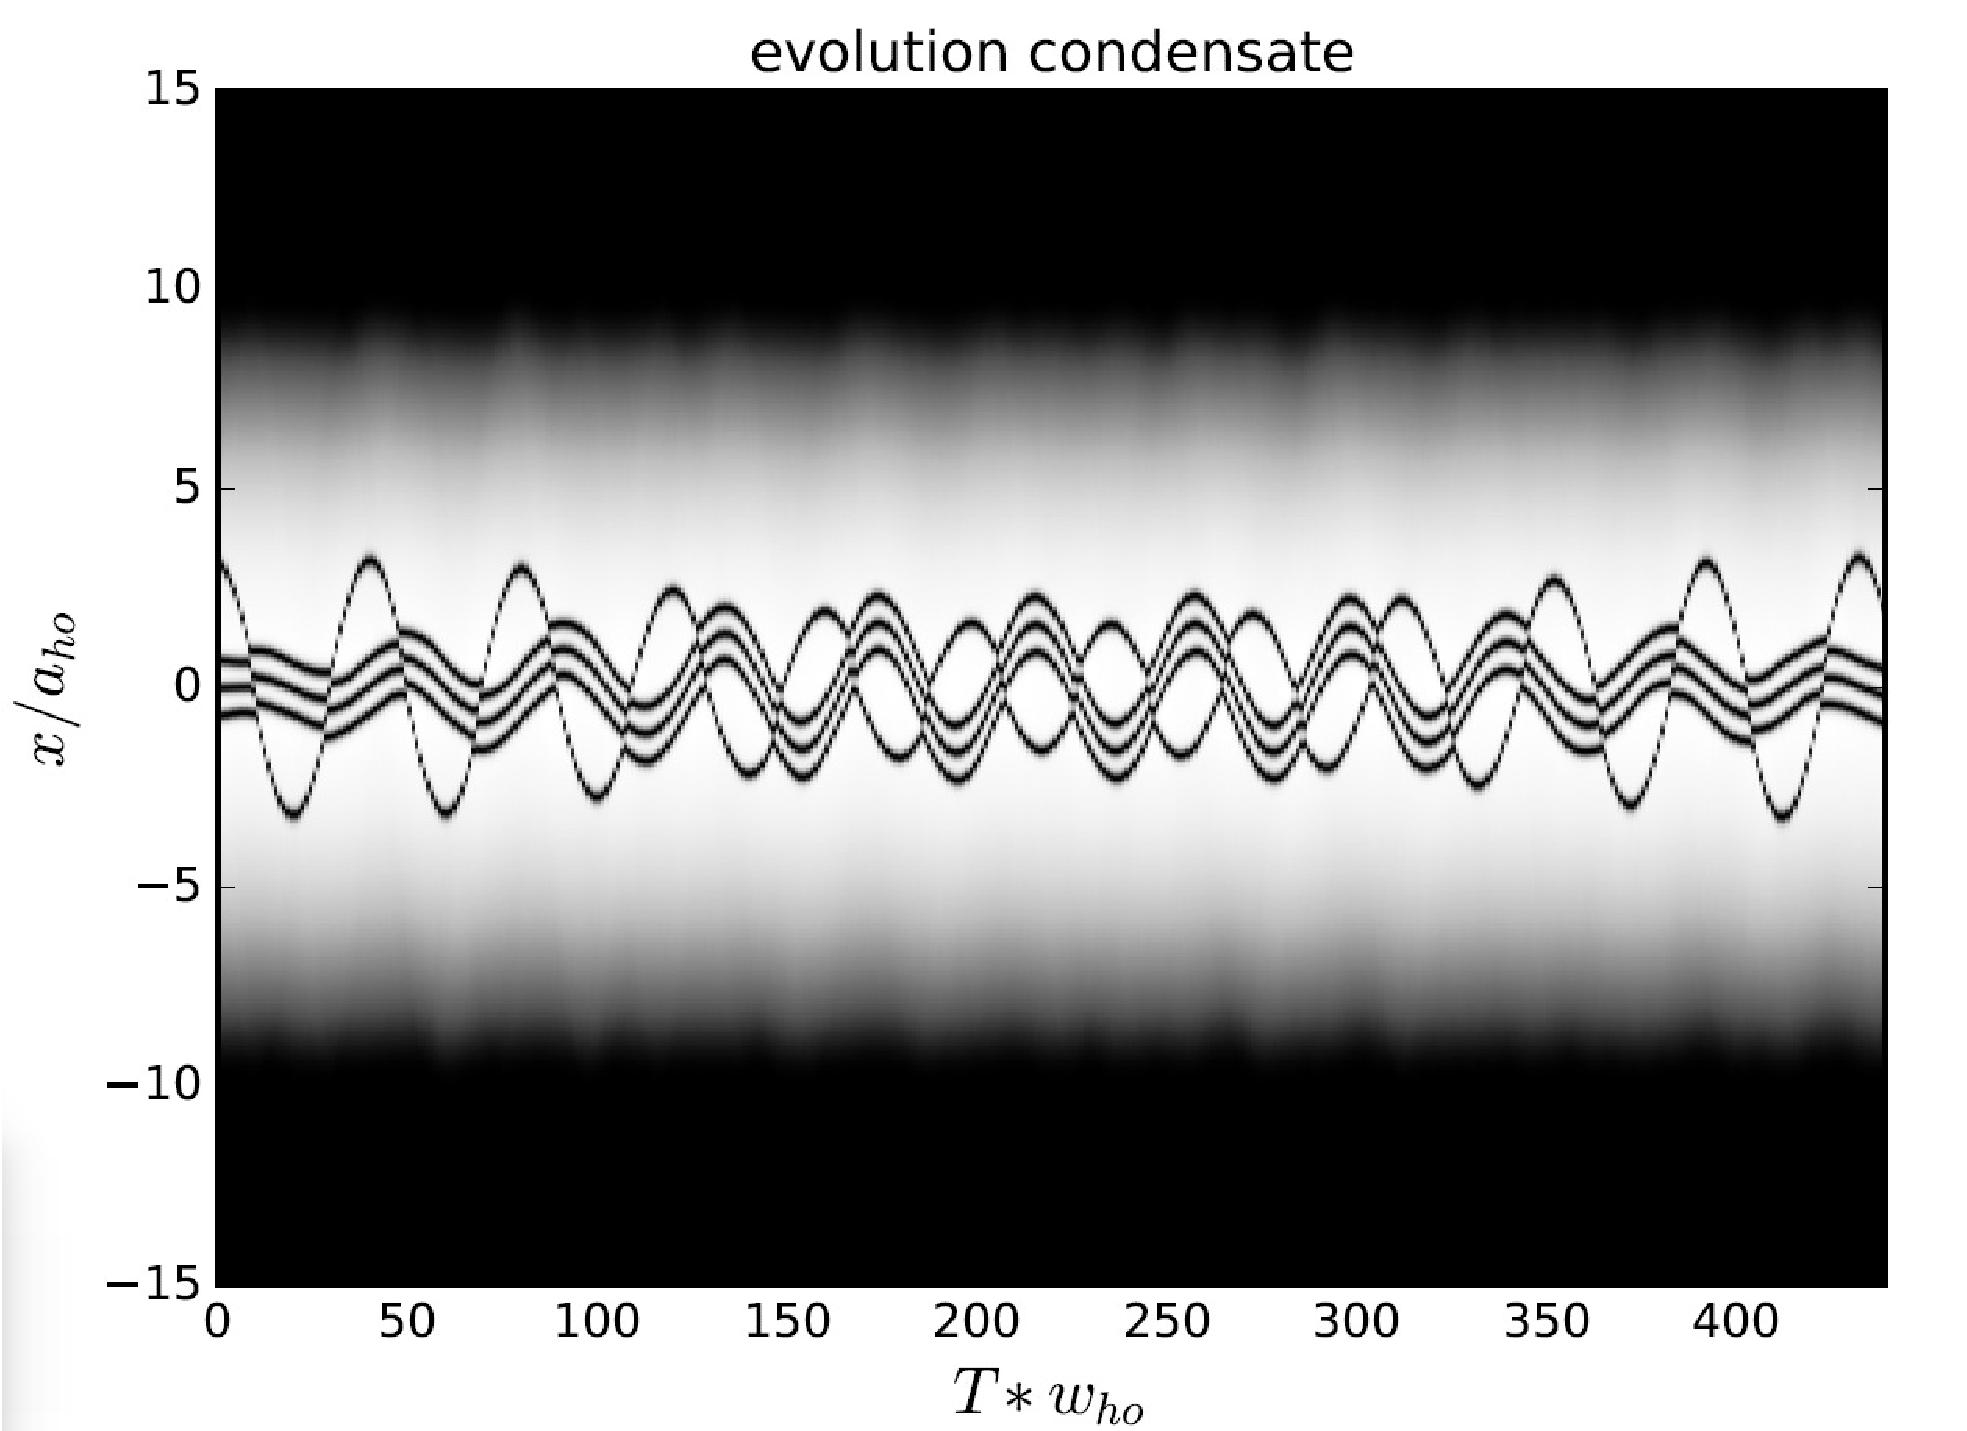
\includegraphics[width=0.9\linewidth]{new_crand.pdf}
	\caption{Evoluci\'on de un estado donde podemos observar el efecto del P\'endulo de Newton}
	\label{Fig:new_crand}
\end{figure}

\end{document}